\chapter[Resultados Parciais]{Resultados Parciais}

\section{Protótipo inicial}

A fim de atestar a viabilidade do porte do jogo \textit{Traveling Will}, desenvolvido inicialmente para PC, para a plataforma \textit{Nintendo Game Boy Advance}, foi feita uma versão funcional do menu original do jogo, já testada em um \textit{Nintendo DS} (como explicado na seção \ref{console} do capítulo \ref{metodologia}). Para isso, a principal ferramenta utilizada foi a \textit{libtonc}\footnote{\textit{libtonc}, disponível em \url{http://www.coranac.com/files/tonc-code.zip}}, que nessa versão inicial fez o papel de engine do jogo.

Abaixo é possível comparar o menu principal do jogo original com o protótipo implementado sendo executado em um emulador de \textit{Game Boy Advance}:

\begin{figure}[H]
 \centering 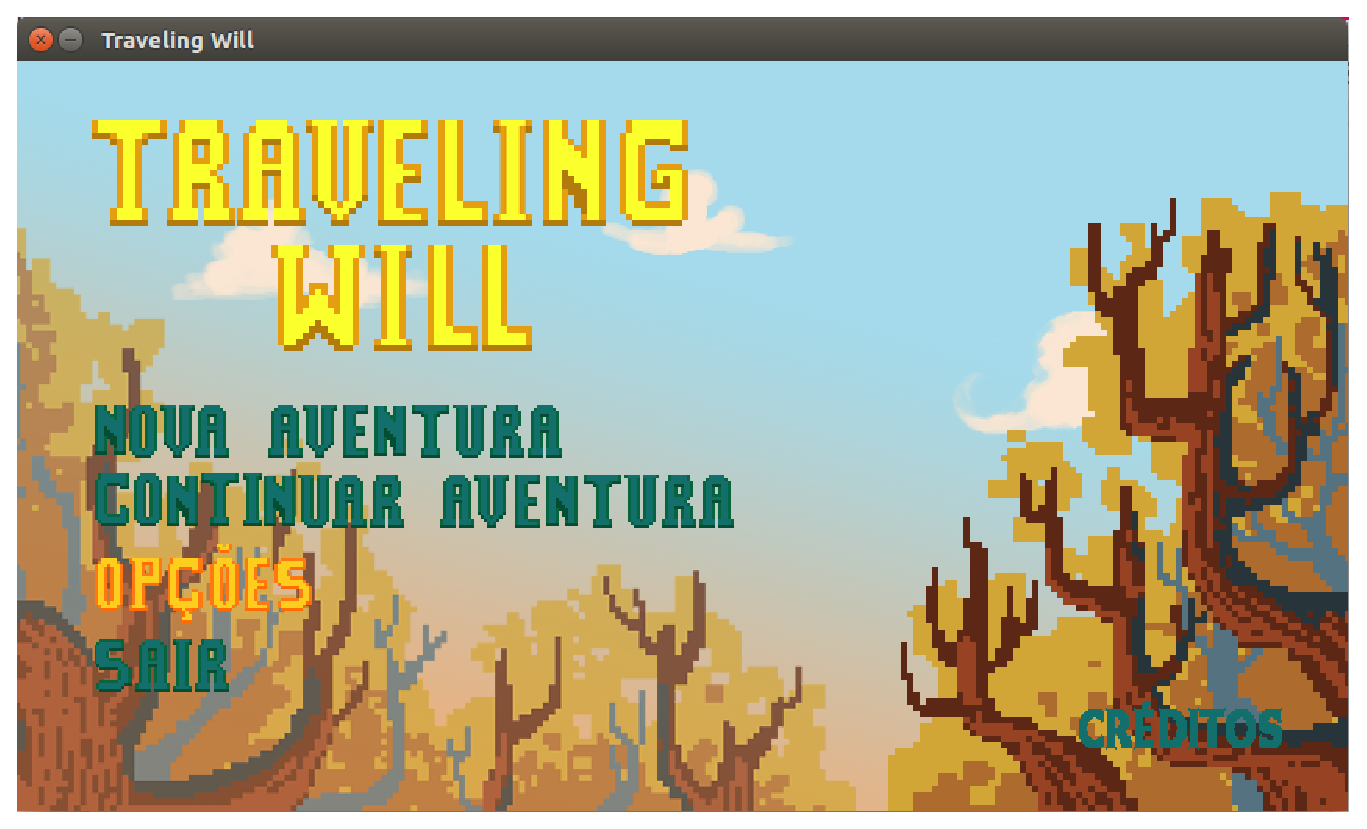
\includegraphics[keepaspectratio=true,scale=0.6]{figuras/tw-original-1.eps}
   \caption[Jogo original sendo executado em um PC]
    {Jogo original sendo executado em um PC. Fonte: \textit{Autores}.}
   \label{tw-original-1}
\end{figure}

\begin{figure}[H]
 \centering 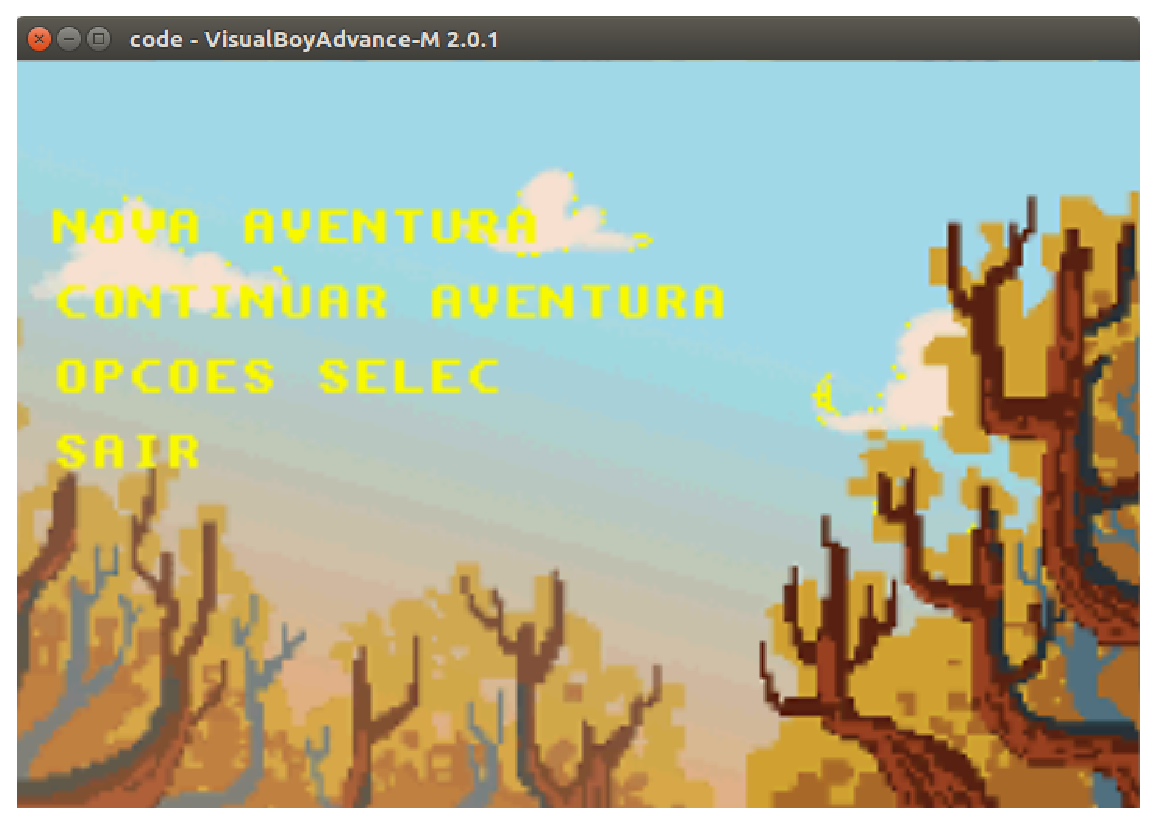
\includegraphics[keepaspectratio=true,scale=0.6]{figuras/tw-gba-1.eps}
   \caption[Protótipo sendo executado no emulador de GBA]
    {Protótipo sendo executado no emulador de GBA. Fonte: \textit{Autores}.}
   \label{tw-gba-1}
\end{figure}

O protótipo desenvolvido está disponível no seguinte repositório: \url{https://github.com/traveling-will-gba/game}

\section{Desenvolvimento da \textit{engine}}

Logo após a finalização do protótipo inicial, foi iniciado o desenvolvimento da \textit{engine} responsável por substituir a \textit{libtonc} e gerenciar os recursos do jogo. Ela foi desenvolvida contendo os seguintes módulos: vídeo, audio, \textit{input} e física. Cada um dos módulos foi desenvolvido tendo como base a \textit{ijengine}... FIXME: Explicar o que é a ijengine.

\subsection{Módulo de \textit{input}}

Os estados dos botões do GBA ficam salvos em um registrador. Cada um desses estados é representado por um \textit{bit} no valor guardado por esse registrador. Sempre que um botão é apertado, o GBA automaticamente troca o valor guardado nesse registrador de tal forma que o \textit{bit} que representa o botão em questão passe a possuir valor 0. De forma similar, quando o botão é solto, o valor contido no \textit{bit} em questão é modificado para 1, seu valor padrão. Sendo assim, a checagem dos estados pode ser realizada facilmente utilizando \textit{bitmasks}. Por exemplo, caso se deseje checar um botão representado pelo \textit{bit} 2 (com a contagem começando em 0), basta pegar o resultado do \textit{AND} binário entre o valor guardado no registrador e a potência de 2 que possui como expotente o \textit{bit} em questão (4, nesse exemplo). Abaixo é possível vizualizar no código do módulo de \textit{input} a definição das constantes que representam os botões, assim como a função utilizada para checar o estado de cada um deles:

\begin{minted}[frame=lines, linenos]
{c++}
#ifndef INPUT_H
#define INPUT_H

#include <stdbool.h>
#include "base_types.h"

#define BUTTON_A 1
#define BUTTON_B 2
#define BUTTON_SELECT 4
#define BUTTON_START 8
#define BUTTON_RIGHT 16
#define BUTTON_LEFT 32
#define BUTTON_UP 64
#define BUTTON_DOWN 128
#define BUTTON_R 256
#define BUTTON_L 512

#define N_BUTTON 10

int pressed_state[N_BUTTON];

void check_buttons_states();
bool pressed(int button);

#endif
\end{minted}
\makebox[\linewidth]{Cabeçalho do módulo de input. Fonte: \textit{Autores}.}
\vspace{\onelineskip}

\begin{minted}[frame=lines, linenos]
{c++}
#include "input.h"

volatile unsigned int *buttons_mem = (volatile unsigned int *)0x04000130;

void check_buttons_states() {
    for(int i = 0; i < N_BUTTON; i++) {
        pressed_state[i] = !((*buttons_mem) & (1 << i));
    }
}

bool pressed(int button) {
    return pressed_state[button];
}
\end{minted}
\makebox[\linewidth]{Código fonte do módulo de input. Fonte: \textit{Autores}.}
\vspace{\onelineskip}

Abaixo é possível visualizar um teste implementado para checar o pressionamento dos botões do GBA. Para cada botão pressionado um \textit{pixel} vermelho aparece na tela. Na imagem abaixo, os botões B, R, \textit{LEFT}, \textit{RIGHT} e \textit{START} estão sendo pressionados simultaneamente.

\begin{figure}[H]
 \centering 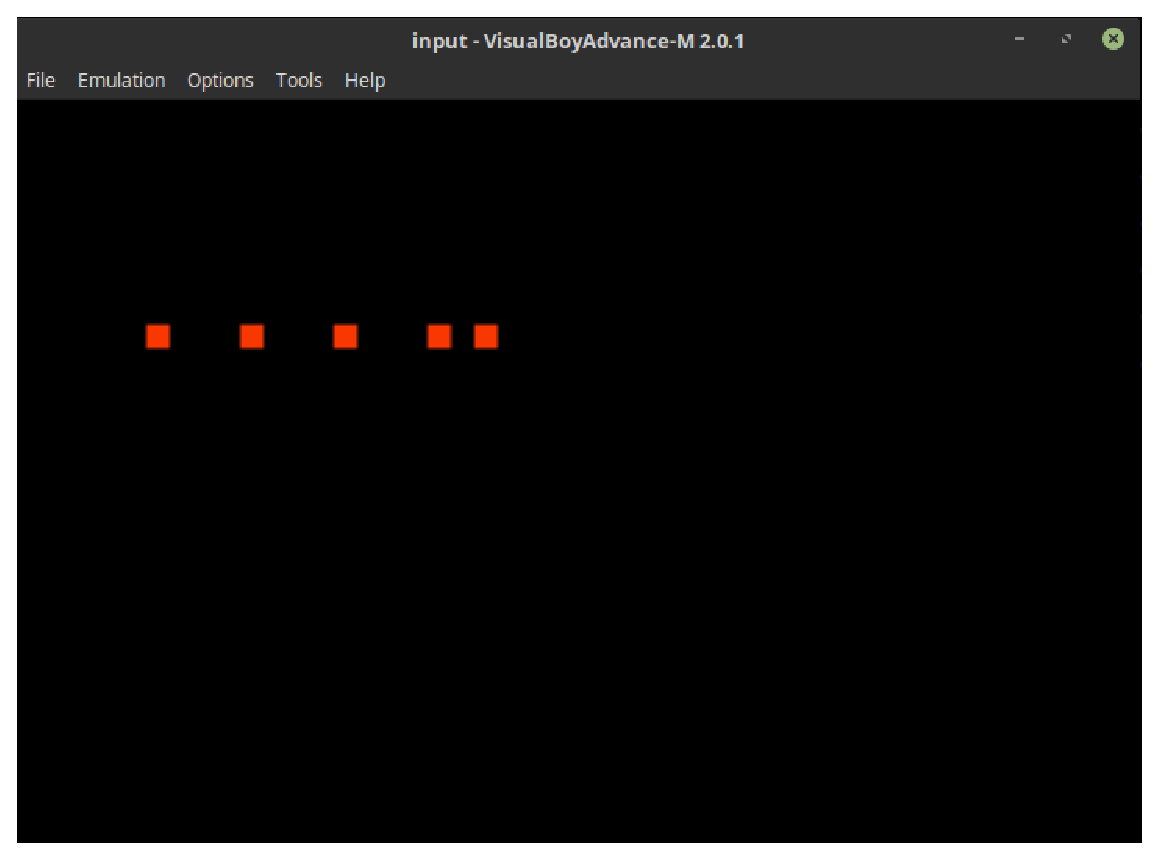
\includegraphics[keepaspectratio=true,scale=0.6]{figuras/demo-input.eps}
   \caption[Demonstração do pressionamento de botões no emulador]
    {Teste de pressionamento de botões no emulador. Fonte: \textit{Autores}.}
   \label{demo-input}
\end{figure}

Abaixo se encontra o código fonte escrito para a realização deste teste:

\begin{minted}[frame=lines, linenos]
{c++}
#include "video.h"
#include "input.h"

#define RED 0x0000FF

unsigned short *vid_mem = (unsigned short *)0x6000000;

int main() {
    reset_dispcnt();
    set_video_mode(3);
    set_background_number(2);

    while(1) {
        check_buttons_states();

        for(int i=0;i<=9;i++){
            if (pressed(i)) {
                vid_mem[50 * 240 + i * 10] = RED;
            } else {
                vid_mem[50 * 240 + i * 10] = 0;
            }
        }
    }

    return 0;
}
\end{minted}
\makebox[\linewidth]{Código fonte do teste de \textit{input}. Fonte: \textit{Autores}.}
\vspace{\onelineskip}

\subsection{Módulo de vídeo}

O módulo de vídeo é responsável pelo controle do modo de vídeo, dos \textit{backgrounds} e da renderização das \textit{sprites}.

Para gerenciar a renderização das \textit{sprites} foi desenvolvida uma classe chamada \textit{Texture}. Ela foi planejada de forma a não apenas copiar os dados da imagem para a região de memória apropriada, mas também permitir a animação das \textit{sprites} de uma textura e controlar os metadados das imagens renderizadas no jogo.

A seguir, será explicado, com o auxílo de trechos do código, o funcionamento dos principais elementos dessa classe.

Inicialmente, é necessário explicar os construtores dessa classe.

Logo abaixo, é possível visualizar o código do primeiro construtor. Ele recebe os ponteiros para a paleta de cores e para o vetor de \textit{tiles} utilizados pela imagem, os tamanhos das regiões de memória alocadas pra cada um desses ponteiros e a quantidade de bits por pixel que a imagem utiliza. Cada um desses atributos é guardado na própria classe, e, já nesse construtor, são chamados os métodos \textit{set\_sprite\_pal} e \textit{set\_sprite}, responsáveis por copiá-los para as regiões apropriadas. Por fim, ainda nesse construtor, são setados os índices do \textit{tile base} e da paleta de cores utilizada pela imagem. O cálculo desses índices será explicado logo adiante, nos tópicos dedicados aos métodos \textit{set\_sprite\_pal} e \textit{set\_sprite}.

O segundo construtor funciona de forma similar ao anterior, com a diferença de que em vez de receber todos os atributos da imagem, ele recebe apenas um ponteiro para outra textura. Esse construtor serve para quando se deseja renderizar réplicas de uma mesma textura. Utilizar ele permite que tais texturas compartilhem a paleta de cores e o vetor de \textit{tiles}, fazendo-se necessário alocar espaço apenas para os metadados, que são diferentes pra cada textura.



Para a renderização dos \textit{backgrounds}, foi desenvolvida uma classe que recebe ponteiros para a paleta de cores,  para o vetor de \textit{tiles} e para o mapa de \textit{tiles} utilizados pelo \textit{background}, assim como os tamanhos das regiões alocadas pra cada um desses ponteiros. Assim que é instanciada, essa classe calcula qual o melhor \textit{charblock} e o melhor \textit{screenblock} para guardar os \textit{tiles} e o mapa de \textit{tiles}, respectivamente. Vale ressaltar que os \textit{charblocks} e \textit{screenblocks} compartilham a mesma região de memória e precisam de um espaço contíguo na memória do \textit{GBA} para que o \textit{background} seja renderizado corretamente. Por esse motivo não é recomendado apenas copiá-los para a memória do \textit{GBA} de forma sequencial, já que isso poderia causar um \textit{overlap} entre um \textit{charblock} e um \textit{screenblock}, e também poderia preencher a memória do \textit{GBA} de forma não-ótima, o que pode fazer com que não caibam todos os \textit{backgrounds} necessários para uma ou mais fases do jogo.

A \textit{engine} desenvolvida está disponível no seguinte repositório: \url{https://github.com/traveling-will-gba/game}
